\documentclass{article}
\usepackage{graphicx} % Required for inserting images

\usepackage{multicol}
\usepackage{hyperref}
\usepackage{amsmath,graphicx,varioref,verbatim,amsfonts,geometry,wasysym}
\usepackage{subcaption}
\usepackage{wrapfig}
\usepackage{caption}
\usepackage{accents}

% Document formatting
\setlength{\parindent}{0mm}
\setlength{\parskip}{1.0mm}
\captionsetup{width=0.8\linewidth}

\hypersetup{
    colorlinks=true,
    linkcolor=black,
    filecolor=magenta,      
    urlcolor=blue,
    pdftitle={Oblig 3},
    pdfpagemode=FullScreen,
    }

\title{LABORATORIERAPPORT I STK-FYS1110}
\author{Bastian Eggum Huuse}
\date{Dato !!!!!!!!!!!!!!!}

\begin{document}

\maketitle

\newpage

\section*{Sammendrag}

Skriv dette til slutt!!!!

\newpage

\tableofcontents

\newpage

\section{Lengde, Tid, og Tyngdeakselerasjon}

\subsection{Innledning}

Første eksperiment er delt i 3 forsøk, alle sentrert rundt lengde, tid, og usikkerheter. I første forsøk (Senere referert til som forsøk a) skulle vi måle perioden til et timeglass ved hjelp av stoppeklokke og pendel. I andre forsøk (Senere referert til som forsøk b) skulle vi måle forskjellige størrelser ved to klosser med tre forskjellige
måleinstrumenter. I tredje forsøk (Senere referert til som forsøk c) skulle vi estimere tyngdeakselerasjonen i Oslo, ved hjelp av Foucault-pendelen som står i fysikkbygget.

Formålet bak forsøkene var å bli kjent med hvordan man utfører et eksperiment, hvordan man dokumenterer dette, og bli introdusert til metoder for å estimere usikkerheter og propagere feil. Både lengde og tid er størrelser som introduserer usikkerheter, siden det ikke er mulig å måle dem helt presist. Det er dermed viktig å lære hvordan man kan, tross for disse usikkerhetene, måle så nøyaktig som mulig, og så kunne anslå akkurat hvor nøyaktig beregningene du har gjort er.

Disse forsøkene har også som formål å introdusere oss som studenter til hvordan det er å utføre et eksperiment rent praktisk. Hvor mange målinger man burde ta, hvordan man skal dokumentere prosessen underveis slik at man kan gjenskape det senere, og hvilke deler av eksperimentet man skal prioritere å få gjort, er viktig å lære, og dette første eksperimentet var en introduksjon til akkurat dette. 

\subsection{Material og Metoder}

Til forsøk a trengte vi en pendel for å måle svingninger (se fig 1), et timeglass vi skulle måle perioden av, stoppeklokker for å måle svingetid for pendelen og den totale tiden timeglasset brukte (I dette tilfellet brukte vi mobiltelefonene våre), og en meterstokk for å måle pendelens lengde.

Først tok vi mål av pendelens lengde, fra opphengspunkt til opphengspunkt. Så fant vi lengden av halve pendelmassen, og la disse to målene sammen for å finne lengden på hele pendelen (Vi propagerte også feilene for disse).

En av oss løftet pendelen vekk fra bunnpunktet, og slapp den slik at den begynte å svinge. Samtidig snudde en annen på gruppa timeglasset slik at den hvite siden pekte nedover, og vi startet stoppeklokkene våre. Vi gjorde hele denne prosessen to ganger.

Så, for å finne pendelens svingetid, løftet vi pendelen til samme punkt, og slapp den mens vi startet stoppeklokkene våre. Hver gang pendelen hadde svinget en hel periode, trykket vi på "runde" slik at vi lagret tiden for hele den nåværende perioden, uten at stoppeklokken stoppet å telle. Vi gjorde dette for 50 perioder. Vi sammenliknet våre mål med den teoretiske svingetiden, som vi fant ved:

\begin{align}
    T =2\pi\sqrt{\frac{L}{g}}\label{TFormula}
\end{align}

Der g = $9.82$ (gitt fra oppgavebeskrivelsen), og L er lengden vi har målt. Fra målingene våre plottet vi også histogram og regnet ut snitt og standardfeil i python.
\bigskip


Til forsøk b trengte vi målestokk, skyvelære, og lasermåler. Vi trengte også de to klossene vi skulle måle tykkelsen av (se fig 1), fra nå av referert til som kloss A og kloss B, der A er tykkere enn B.

Først skulle vi måle tykkelsen på begge klossene, ved hjelp av alle tre instrumentene. Vi tok mål så presist vi kunne, både ved oppsett av instrumentene og ved avlesning. Vi stilte opp målestokken inntil klossen vi skulle måle, og en av oss holdt den rett mens en annen leste av. Når vi skulle ta mål med skyvelæren, plasserte vi klossen i skyvelærens "klør" [DÅRLIG TERMINOLOGI], lukket den så tett på klossen som mulig, og leste av. Vi fant ut at lasermåleren har en grense på hvor korte distanser den kan måle, så vi kunne ikke måle klossens tykkelse direkte. Vi kom rundt dette ved å måle en lenger distanse, avstanden fra bunnen av bordet vi satt ved til gulvet, og så målte vi denne samme distansen etter vi hadde lagt klossen inn under laseren. Vi kunne da finne klossens tykkelse ved å se trekke det andre målet fra det første (dette introduserer enda en usikkerhet, som dokumenteres mer resultater-delen). Vi brukte de forskjellige målene våre for tykkelsene til kloss A og B, til å estimere differansen mellom tykkelsene deres.

\bigskip \hfil
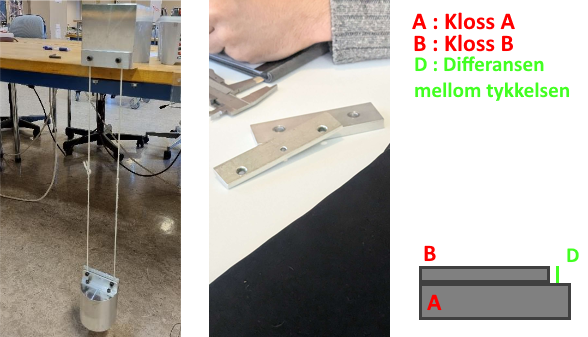
\includegraphics[scale = 0.8]{Figurer/Lab_Fig_1.png} 
\captionof{figure}{Pendel vi brukte i forsøk a (venstre), Klossene brukt i forsøk b (sentrum), og plassering av klossene i andre del av forsøk b (høyre).}
\par \bigskip

Så skulle vi måle differansen i tykkelse direkte, med målestokk og skyvelære. Vi stablet kloss B på toppen av kloss A (se fig 1), og tok mål. Med målestokken gjorde vi samme prosess som tidligere, mens med skyvelæren brukte vi "bunnen" [DÅRLIG TERMINOLOGI] til å måle differansen.\bigskip

Til forsøk c trengte vi lasermåleren, stoppeklokke (vi brukte igjen mobiltelefoner), Focault-pendelen som står i fysikkbygget, og diverse bøker av forskjellige størrelser.

Først målte vi tiden pendelen brukte på å svinge en hel periode, fra sentrum til sentrum. Vi gjorde dette alle tre, og fikk dermed 3 mål.

Så skulle vi finne lengden på pendelen. Vi stablet bøkene våre på toppen av hverandre, og plasserte lasermåleren på toppen av stabelen. Så pekte vi lasermåleren inn mot der pendelen når sitt laveste punkt. Så justerte vi høyden på stabelen fram til lasermåleren traff rett over pendelmassens midtpunkt (Vi ønsker å måle fra pendelmassens sentrum, men vi må ta lasermålerens tykkelse i betraktning. Derfor finner vi posisjonen litt over pendelmassens sentrum). Så snudde vi lasermåleren opp, for å måle distansen fra pendelmassens sentrum til taket. Til slutt, la vi til distansen mellom taket og der pendelen er hengt opp, som ble gitt i oppgaven.

Så estimerte vi vinkelens utslag, for å sjekke om småvinkelapproksimasjonen er gyldig. Vi tok et grovt mål fra den ene siden av gjerdet til den andre, og delte denne lengden i to (se fig 2). Vi kunne så finne tangens til det største vinkelutslaget ved å dele denne horisontale lengden på pendelens lengde, og så finne vinkelutslaget.

\hfil
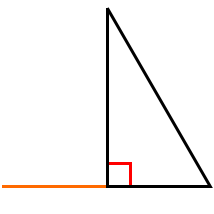
\includegraphics[scale = 0.8]{Figurer/Pendel_Lab1_c.png} 
\captionof{figure}{Lengder vi brukte til å anslå Foucault-pendelsens utslag. Her er summen av de to horisontale lengdene lik lengden fra den ene siden av gjerdet til den andre, mens den vertikale linjen er lengden på pendelen.}
\par \bigskip

Til slutt estimerte vi akselerasjonen i oslo ved bruk av uttrykket 

\begin{align}
    \hat{g} = \frac{4\pi^2l_p}{T^2}\label{ghat}
\end{align}

og sammenliknet det med $g = 9.82$, som vi vet er tyngdeakselerasjonen i oslo.
\bigskip

Til alle forsøkene brukte vi flere formler til å estimere feil, hovedsakelig

\begin{align}
    u_f = \sqrt{u_x^2 +u_y^2}\label{au}
\end{align}


som estimerer usikkerheten i summen av to usikre mål. Mer generelt anvendte vi 

\begin{align}
    u_f^2 = \left(\frac{\delta f}{\delta x} u_x\right)^2 + \left(\frac{\delta f}{\delta y} u_y\right)^2\label{gu}
\end{align}

for å estimere usikkerheter. Dersom et utrykk inneholder fler enn 2 variabler med usikkerheter, kan man da legge inn flere ledd i utrykket over.

\subsection{Resultater}

\subsubsection*{Forsøk a}

Vi fikk følgende mål for pendelens lengde:

\begin{center}
\begin{tabular}{ | c | c | c | }
    \hline
    & Lengde (cm) & Usikkerhet i avlesning (cm)\\ 
    \hline
    $l_o$ (mellom opphengspunkter) & 52.45 & 0.2\\ 
    \hline
    $l_m$ (pendelmassen) & 10.15 & 0.1\\ 
    \hline
\end{tabular}
\captionof{table}{Målinger av pendelens lengde}
\end{center}

for å estimere lengden av hele pendelen $l_p$, fra opphengspunkt til pendelmassens sentrum, må legge sammen $l_0$ og $\frac{l_m}{2}$. Dette gir oss $l_p = 62.6$. For å finne usikkerheten, bruker vi formel \ref{au}:

\begin{align}
    u_{l_p} = \sqrt{u_{l_o}^2 + u_{l_m}^2 + 2u_{ledd}^2 + 2u_{skala}^2}
\end{align}

her er $u_{ledd} = 0.5 \cdot 10^{-3} m$ og $u_{skala} = 0.5 \cdot 10^{-3} m$. Disse er usikkerhetene i målestokken, og ble gitt i oppgaveteksten. Dette gir oss 

\begin{align*}
    u_{l_p} &= \sqrt{\left(0.2\cdot10^{-2}\right)^2 + \left(0.1\cdot10^{-2}\right)^2 + \left(0.5\cdot10^{-3} \right)^2 + \left(0.5\cdot10^{-3} \right)^2} \; m\\
    &\approx 0.0023 \; \text{m}\\
    &= 0.23 \; \text{cm}
\end{align*}

Vi har altså $l_p = 62.6$ cm, og $u_{l_p} = 0.23$ cm. \bigskip

Som tidligere nevnt, målte vi timeglassets periode to ganger. Resultatet av disse målingene er som følger: 

\begin{center}
\begin{tabular}{ | c | c | c | }
    \hline
    & Første måling (sekunder) & Andre måling (sekunder)\\ 
    \hline
    Klokke 1 & 183.97 & 185.19 \\ 
    \hline
    Klokke 2 & 184.02 & 183.31\\ 
    \hline
    Klokke 3 & 183.94 & 183.91 \\ 
    \hline
\end{tabular}
\captionof{table}{Timeglassets periode målt med tre stoppeklokker}
\end{center}

\begin{center}
\begin{tabular}{ | c | c | c | }
    \hline
    & Første måling (antall) & Andre måling (antall)\\ 
    \hline
    Antall Svingninger & 122 & 120.5\\ 
    \hline
\end{tabular}
\captionof{table}{Timeglassets periode målt i antall perioder}
\end{center}

[SETT INN USIKKERHETER FOR DETTE HER!!!!] \bigskip

De 50 målingene tatt av pendelens svingetid ligger vedlagt i \nameref{Vedlegg}. Vedlagt ligger også program \ref{Svingehistogram.py}, som ble brukt til å plotte disse målingene. Dette produserte følgende histogram:

\begin{center}
    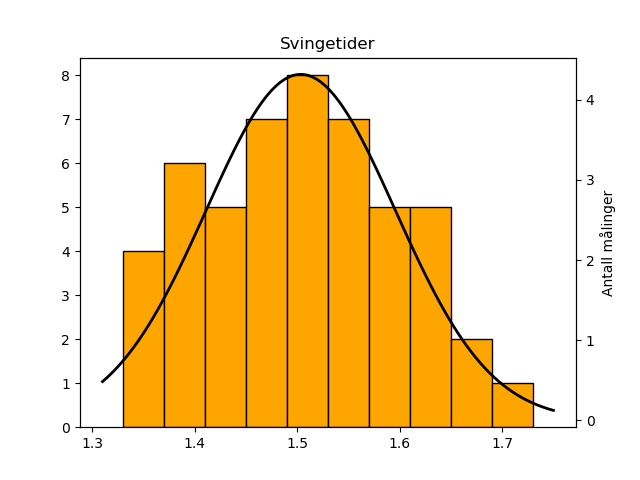
\includegraphics[scale = 0.6]{Figurer/Lab_1_Hist_1.png} \label{Hist_1}
    \captionof{figure}{Histogram av pendelens svingetider, sammen med den teoretiske normalfordelingen}
\end{center}

[KOMMENTER DETTE HER!!!]\bigskip

Fra programmet fikk vi også gjennomsnitt og standardfeil.

\begin{center}
\begin{tabular}{ | c | c | }
    \hline
    & Tid (sekunder)\\
    \hline
     $\bar{t}$ & 1.50\\
    \hline
     $SEM(t)$ & 0.0130\\
    \hline
\end{tabular}
\captionof{table}{Snitttid og standardfeil}
\end{center}

Vi kan sammelikne disse tallene med den teoretiske svingetiden vi får fra formel \ref{TFormula}, og så kan vi bruke formel \ref{gu} for å finne usikkerhetene.

\newcommand{\alignref}[1]{\;\;\;\text{$\left(\ref{#1}\right)$}}

\begin{align*}
    T =2\pi\sqrt{\frac{L}{g}} \alignref{TFormula}\\
    u_f^2 = \left(\frac{\delta f}{\delta x} u_x\right)^2 + \left(\frac{\delta f}{\delta y} u_y\right)^2 \alignref{gu}
\end{align*}

Dette gir oss

\begin{center}
\begin{tabular}{ | c | c | }
    \hline
    & Tid (sekunder)\\
    \hline
     $\accentset{*}{t}$ & 1.59\\
    \hline
     $u_{\accentset{*}{t}}$ & 0.0540\\
    \hline
\end{tabular}
\captionof{table}{Teoretisk tid og usikkerhet}
\end{center}

Vi kan så plotte denne teoretiske tiden sammen med histogrammet.

\begin{center}
    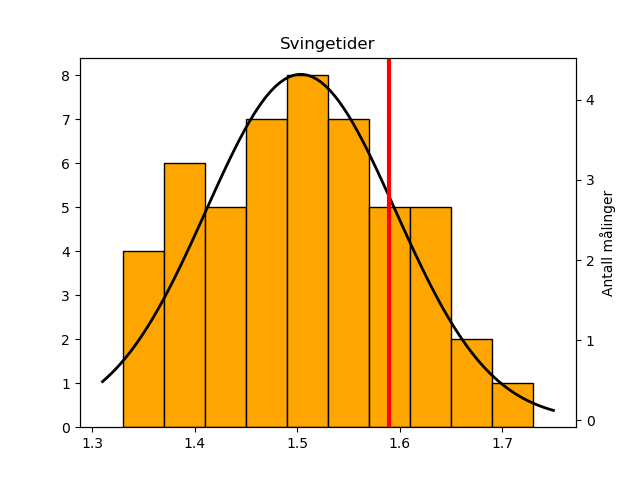
\includegraphics[scale = 0.6]{Figurer/Lab_1_Hist_2.png} \label{Hist_2}
    \captionof{figure}{Histogram av pendelens svingetider, sammen med den teoretiske normalfordelingen og den teoretiske svingetiden.}
\end{center}

\subsubsection*{Forsøk b}

Vi fikk følgende mål og usikkerheter for tykkelsene på klossene (Den totale usikkerheten er listet opp som $u_{total}$, som vi fant ved hjelp av formel \ref{au}):

\begin{center}
\begin{tabular}{ | c | c | c | c | c | c |}
    \hline
    & $l_a$ & $l_b$ & $u_{avles}$ & $u_{skala}$ & $u_{total}$\\
    \hline
     Skyvelære & 8.0  & 5.0  & 0.05 & 0.05 & 0.07\\
    \hline
     Målestokk & 8.0 & 5.0 & 0.5 & 0.5 & 0.9\\
     \hline
\end{tabular}
\captionof{table}{Mål og usikkerheter, gjort ved Skyvelære og målestokk, for tykkelsene på klossene (alt er målt i millimeter)}\label{table6}
\end{center}

\begin{center}
\begin{tabular}{ | c | c | c | c | c | c | c | c | c |}
    \hline
    & $l_t$ & $l_{t-a}$ & $l_{t-b}$ & $l_a$ & $l_b$ & $u_{avles}$ & $u_{skala}$ & $u_{total}$\\
    \hline
     Lasermåler & 719 & 709 & 713 & 10 & 6.0  & 0.0 & 2.0 & 2.8\\
    \hline
\end{tabular}
\captionof{table}{Mål og usikkerheter, gjort ved lasermåler, for tykkelsene på klossene (alt er målt i millimeter)}\label{table7}
\end{center}

I den totale usikkerheten til målestokken, måtte vi også ta med målestokkens $u_{ledd} = 0.5$mm, som ble gitt i oppgaveteksten.

Som nevnt var prosessen for å måle tykkelsene med lasermålet noe mer komplisert enn med de andre instrumentene. Vi måtte altså introdusere lengdene $l_t,l_{t-a}$, og $l_{t-b}$, som er lengdene fra bordet til gulvet, og fra bordet til gulvet etter vi hadde lagt klossene inn under laseren. Dette la til usikkerheter, som vi fant ved hjelp av formel \ref{au}.

\begin{align*}
    u_f = \sqrt{u_x^2 +u_y^2} \alignref{au}
\end{align*}

vi kan så finne $\Delta_{a-b}$ for alle målemetodene, og så, igjen ved hjelp av formel \ref{au}, finne usikkerhetene:

\begin{center}
\begin{tabular}{ | c | c | c |}
    \hline
    & $\Delta_{a-b}$ & $u_{\Delta_{a-b}}$\\
    \hline
     Skyvelære & 3.0 & 0.099\\
    \hline
     Målestokk & 3.0 & 1.3\\
     \hline
     Lasermåler & 4.0 & 4.0\\
     \hline
\end{tabular}
\captionof{table}{Estimerte differanser i tykkelse, med usikkerheter (i millimeter)}\label{table8}
\end{center}

Så sammmenlikner vi med de målte differansene $\Delta_{a-b}$:

\begin{center}
\begin{tabular}{ | c | c | c | c | c |}
    \hline
    & $\Delta_{a-b}$  & $u_{avles}$ & $u_{skala}$ & $u_{total}$\\
    \hline
     Skyvelære & 3.2  & 0.05  & 0.05 & 0.07\\
    \hline
     Målestokk & 3.0 & 0.5 & 0.5 & 0.9 \\
     \hline
\end{tabular}
\captionof{table}{Målte differanser i tykkelse, med usikkerheter, gjort ved Skyvelære og målestokk (i millimeter)}\label{table9}
\end{center}

\subsubsection*{Forsøk c}

Vi fikk følgende mål på pendelens periode:

\begin{center}
\begin{tabular}{ | c | c |}
    \hline
    & tid (sekunder)\\
    \hline
    Klokke 1 & 7.45\\
    \hline
    Klokke 2 & 7.54\\
    \hline
    Klokke 3 & 7.58\\
    \hline
\end{tabular}
\captionof{table}{Målte perioder for Foucault-pendelen}
\end{center}

 Senere vil vi bruke snittet av disse, $\overline{t} = 7.52$s til å beregne tyngdeakselerasjonen, sammen med $SEM(t) = 0.0314$s, som usikkerheten (Denne usikkerheten ble funnet via et lite program, som er lagt ved som vedlegg \ref{SEM.py})
\medskip

Så fikk vi følgende mål for pendelens høyde:

\begin{center}
\begin{tabular}{ | c | c | c |}
    \hline
    & Lengde (meter) & Usikkerhet (meter)\\
    \hline
    $l_t$ & 13.714 & 0.05\\
    \hline
    $l_f \; \text{(gitt i oppgaven)}$ & 0.64  & 0.08\\
    \hline
    $l_p = l_t + l_f$ & 14.354 & 0.094\\
    \hline
\end{tabular}
\captionof{table}{Målt lengde for Foucault-pendelen}
\end{center}

Når vi skulle sjekke om småvinkelapproksimasjonen gjelder, målte vi $l_x = 2.53$ meter fra en side av gjerdet rundt pendelen til den andre (Vi regner ikke med usikkerheter her.). Vi deler denne lengden på to, og kan da finne det teoretisk største vinkelutslaget:

\begin{align*}
    \theta &= arctan\left(\frac{\frac{l_x}{2}}{l_p}\right)\\
    &= arctan\left(\frac{1.265}{14.354}\right)\\
    &= 5.0363^{\circ}
\end{align*}

Pendelen vil aldri svinge helt ut til gjerdet, så vi vet at det ordentlige største vinkelutslaget vil være mindre enn dette. Som regel bruker man ca $10^{\circ}$ som grensen for småvinkelapproksimasjonen, så vi kan si med godt grunnlag at småvinkelapproksimasjonen gjelder.\bigskip

Til slutt, estimerer vi tyngdeakselerasjonen ved bruk av formel \ref{ghat}

\begin{align*}
    \hat{g} &= \frac{4\pi^2l_p}{\overline{t}^2} \alignref{ghat}\\
    &= \frac{4\pi^214.354}{7.52}\\
    &= 10.02
\end{align*}

Så finner vi usikkerheten ved bruk av formel \ref{gu}:

\begin{align*}
    u_f^2 = \left(\frac{\delta f}{\delta x} u_x\right)^2 + \left(\frac{\delta f}{\delta y} u_y\right)^2 \alignref{gu}
\end{align*}

\begin{align*}
    u_{\hat{g}}^2 &= \left(\frac{\delta \hat{g}}{\delta \overline{t}} u_{\overline{t}}\right)^2 + \left(\frac{\delta \hat{g}}{\delta l_p} u_{l_p}\right)^2\\
    &=  \left(\frac{-8\pi^2l_p}{\overline{t}^3} u_{\overline{t}}\right)^2 + \left(\frac{4\pi^2}{\overline{t}^2} u_{\overline{t}}\right)^2\\
    &= 0.0113\\
    u_{\hat{g}} &= \sqrt{0.0113}\\
    &= 0.106
\end{align*}

Dermed har vi at $\hat{g} = 10.02$ m/$s^2$, og $u_{\hat{g}} = 0.106$ m/$s^2$.

\subsection{Diskusjon}

Disse forsøkene var de første vi gjorde, og vi var relativt uerfarne når vi gjennomførte dem. Jeg mener at vi i løpet av forsøkene ble bedre på både hvordan utføre forsøkene rent praktisk, men også på hvordan vi skulle tenke rundt dem. \medskip

I forsøk a kan vi se at den teoretiske svingetiden er mindre sikker enn den empiriske. Siden vi kun har ett mål å gå på når vi estimerer den teoretiske svingetiden, gir det mening at denne er mindre sikker. På figur \ref{Hist_2} kan vi også se at det empiriske snittet er forskjøvet litt mot høyre (langs tidsaksen). Siden alle mål brukt i dette histogrammet er tatt av meg, antar jeg at det systematiske avviket kommer av menneskelige feil, altså at jeg konsekvent tar for korte målinger.\medskip

I forsøk b ser vi at Skyvelæren og Målestokken måler tykkelsen på klossene ganske nøyaktig, mens Lasermåleren er dårlig egnet til å måle så korte distanser. I tabell \ref{table7} kan vi se at Lasermåleren har hele 2.8 mm usikkerhet, som er mye sammenliknet med målestokkens 0.9 mm og skyvelærens 0.07 mm vi kan se i tabell \ref{table6}. Mye av denne usikkerheten kommer fra at vi måtte måle tykkelsen i flere steg når vi brukte lasermåleren, men dette viser igjen at lasermåleren ikke er best egnet til å måle så korte distanser.

For differansen mellom tykkelsene, ser vi at å måle direkte som regel gir et sikrere mål. I tabell \ref{table9} ser vi at målet tatt med målestokk samsvarer med estimatene i tabell \ref{table8}, men at det direkte målet er mindre usikkert. Det direkte målet med skyvelæren er også mer nøyaktig, men samsvarer ikke helt med estimatet. Siden alle andre mål peker mot 3.0 (hvis vi ser bort fra lasermålingen) antar jeg det er en feil i denne målingen, jeg vil tro en avlesingsfeil, og om jeg skulle utført forsøket igjen ville jeg forsøkt enda mer å ta nøyaktige mål.
Siden den direkte målingen har lavere usikkerheter, mener jeg at denne er den beste metoden for å finne differansen.\medskip

I forsøk c, brukte vi snitt og standardfeil når vi skulle regne med den målte tiden, selv om vi bare hadde tre målinger. Dersom jeg skulle gjort forsøket igjen, ville jeg tatt flere målinger av pendelens svingetid, for å få et mer nøyaktig mål. Vårt endelige estimat $\hat{g} = 10.02$ m/$s^2$, med usikkerheten $u_{\hat{g}} = 0.106$ m/$s^2$, er ikke veldig langt unna den ordentlige Gravitasjonsakselerasjonen i oslo, som er $9.82$ m/$s^2$. For å få et enda bedre estimat, kunne vi som tidligere nevnt tatt flere mål av svingetiden. Måten vi brukte til å estimere pendelens lengde var heller ikke den beste. Jeg er sikker på at det finnes en bedre måte å måle denne lengden på. \medskip

Generelt, mener jeg at målene vi tok var relativt gode, men at det definitivt er mulige forbedringer. Jeg tror at dersom vi fikk gjennomføre forsøkene igjen, med den erfaringen vi har nå, at vi kunne fått mer nøyaktige resultater.

\newpage

\section{Måling av Masse}

\subsection{Innledning}

Andre eksperiment var delt inn i to forsøk, basert på forskjellige måter å måle et objekts masse. 
I det første forsøket (som jeg vil referere til som forsøk d), skulle vi bruke en fjærvekt til å måle elastisk deformasjon. Når det henger et objekt med masse $m$ i fjæren, vil gravitasjonskraften motvirkes av fjærkraften, gitt ved Hookes lov, ($F = k\cdot l$). Dette gir oss at Gravitasjonskraften er proporsjonal med fjærens utstrekning, og siden $G = mg$, der vi antar at $g$ er konstant, har vi at massen er proporsjonal med fjærens utstrekning, og at vi kan bruke fjæren til å anslå et objekts masse. \medskip

I det andre forsøket (videre referert til som forsøk e), skulle vi bruke en harmonisk oscillator til å anslå et objekts masse. Ved å se på hvordan oscillatorens svingetid endrer seg når masse legges til, kan vi anslå endringen i masse, og dermed hvor stor massen til objektet vi la til er. \medskip

Begge disse forsøkene introduserer konseptet kalibrering, altså hvordan man ved hjelp av kjente verdier kan sette opp måleinstrumenter til å måle ukjente verdier. I våre tilfeller bruker vi da altså objekter som vi vet massen til fra før, til å beregne masser vi ikke kjenner til fra før. Vi ønsker også, for begge forsøkene, å anslå et dynamisk område for måleinstrumentene. Dynamisk område er forholdet mellom den største og den minste verdien et instrument kan måle, og viser hvor godt et måleinstrument er til å måle verdier av forskjellige størrelsesordener.

\subsection{Material og Metoder}

Til forsøk d trengte vi en bladvekt til å måle deformasjon (se fig \ref{forsøk_d_fig}), et sett med kalibreringslodd med kjente masser (Våre hadde massene 1g, 10g, 100g, 500g, 1000g, og 2000g), hansker slik at vi ikke la igjen fingeravtrykk på kalibreringsloddene (dette ville ført til at loddene endret masse), og det store loddet med ukjent masse vi ønsker å måle (se fig \ref{forsøk_d_fig}).

\bigskip \hfil
\includegraphics[scale = 0.07]{Figurer/Lab_Fig_d.png} 
\captionof{figure}{Bladvekt (venstre) og lodd med ukjent masse (høyre)} \label{forsøk_d_fig}
\par \bigskip

Vi begynte med å sjekke at loddet vi ønsket å måle var innenfor bladvektens rekkevidde. Vi plasserte loddet i kurven som var festet til bladet på vekten, og sjekket at dette ikke deformet bladet lenger enn det måleuret kunne måle.
Når vi hadde sjekket dette, begynte vi å kalibrere bladvekten. Vi leste av måleuret for mange kombinasjoner av kalibreringsloddene (Hvilke kombinasjoner er spesifisert i \nameref{Resultater_2}). \medskip

Så plottet vi en kalibreringskurve for bladvekten i python, og tilpasset en lineær regresjonsmodell til denne kurven, slik at vi kunne anslå massen til det ukjente loddet. Vi plottet også residualplott og prediksjonsintervall, for å finne usikkerheten i målingen. \bigskip

Til forsøk e trengte vi en harmonisk oscillator, vi brukte en pendel bygget opp av en bladfjær og et lodd (se fig \ref{forsøk_e_fig}). Vi trengte også en stoppeklokke (vi brukte mobiltelefoner), en digital-vekt, unbrakonøkkeler og binderser i varierende størrelser, og tape.

Først tok 20 målinger av pendelens svingetid, i 5 og 5 svingninger om gangen. Så målte vi massen til loddet vi brukte i forsøk d, for å estimere massen til loddet vårt. Vi brukte så følgende formel til å estimere fjærkonstanten.

\begin{align}
    T =2\pi\sqrt{m/k} \label{periodformula}
\end{align}

Så brukte vi samme formel, sammen med følgende formel for å estimere usikkerheten i massen $u_m$. Dette er da den minste endringen i masse vi kan måle.

\begin{align}
    u_f^2 = \left(\frac{\delta f}{\delta x} u_x\right)^2 + \left(\frac{\delta f}{\delta y} u_y\right)^2\label{gu}
\end{align}

Vi teipet sammen umbrakonøkkeler og binderser fram til de hadde masse ca. lik $u_m$, og festet dette til pendelen (se fig \ref{forsøk_e_fig}). Vi målte så pendelens svingetid igjen.

\bigskip \hfil
\includegraphics[scale = 0.07]{Figurer/Lab_Fig_e.png} 
\captionof{figure}{Vår harmoniske Oscillerator (Venstre), og samme oscillerator tilsatt en liten masse ca. lik $u_m$} \label{forsøk_e_fig}
\par \bigskip

Vi repeterte dette med masse ca. lik $2u_m$ og $3u_m$.\medskip

Til slutt plottet vi alle periodemålingene våre sammen i python.


\subsection{Resultater} \label{Resultater_2}

\subsubsection*{Forsøk d}
Vi fikk følgende kalibreringsmål:

\begin{center}
\begin{tabular}{  | c | c |}
    \hline
    Masse (g) & Lengde på deformasjon (mm)\\
    \hline
    0 & 6.16\\
    \hline
    1 & 6.16\\
    \hline
    10 & 6.14\\
    \hline
    100 & 5.93\\
    \hline
    110 & 5.92\\
    \hline
    500 & 4.97\\
    \hline
    510 & 4.96\\
    \hline
    600 & 4.68\\
    \hline
    610 & 4.67\\
    \hline
    1000 & 3.78\\
    \hline
    1010 & 3.76\\
    \hline
    1100 & 3.555 ($\pm 0.005$)\\
    \hline
    1110 & 3.53\\
    \hline
    1500 & 2.69\\
    \hline
    1510 & 2.665 ($\pm 0.005$)\\
    \hline
    1600 & 2.47\\
    \hline
    1610 & 2.455 ($\pm 0.005$)\\
    \hline
    2000 & 1.62\\
    \hline
    2100 & 1.40\\
    \hline
\end{tabular}
\captionof{table}{Lengden lest av måleuret for forskjellige kombinasjoner av kalibreringsloddene}
\end{center}

Vi tilpasset en lineær regresjonsmodell til disse målene (se vedlegg \ref{Kalibreringskurve.py} for kode), og fikk følgende graf og utrykk:

\begin{center}
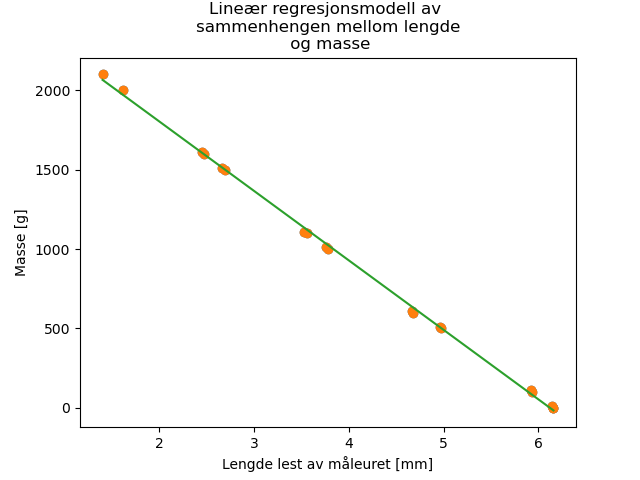
\includegraphics[scale=0.7]{Figurer/Lab_2_regresjon.png}
\end{center}

\begin{align*}
    m(l) &= (2677.847483) + (-437.310226)\cdot l 
\end{align*}
\captionof{figure}{Lineær regresjonsmodell og korresponderende funksjonsutrykk.}
\bigskip

Når vi la aluminiumsloddet i kurven, leste vi av $1.27$ mm på måleuret. Dersom vi setter dette inn i funksjonen vi fant ved regresjonen, får vi at loddet har massen 2122.5 g. Så plottet vi residualer for denne regresjonsmodellen:

\begin{center}
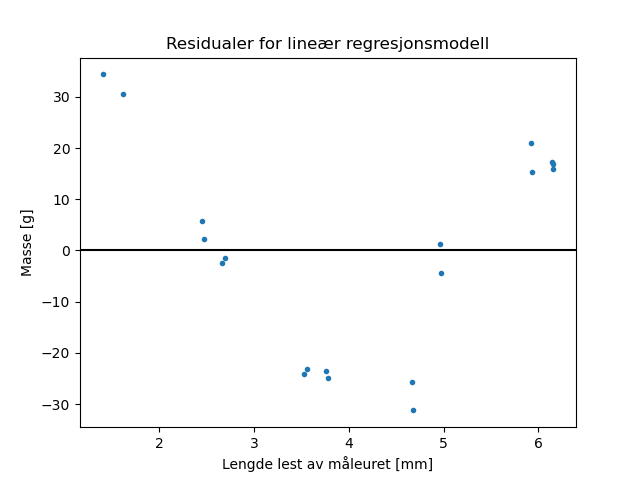
\includegraphics[scale=0.7]{Figurer/Lab_2_Residualer.png}
\end{center}

Vi ser at residualene følger en kurve, der de korteste og lengste lengdene gir store positive avvik, mens lengdene mot midten gir store negative avvik.\medskip

Vi fikk følgende plott for regresjonsmodellens prediksjonsintervall:

\begin{center}
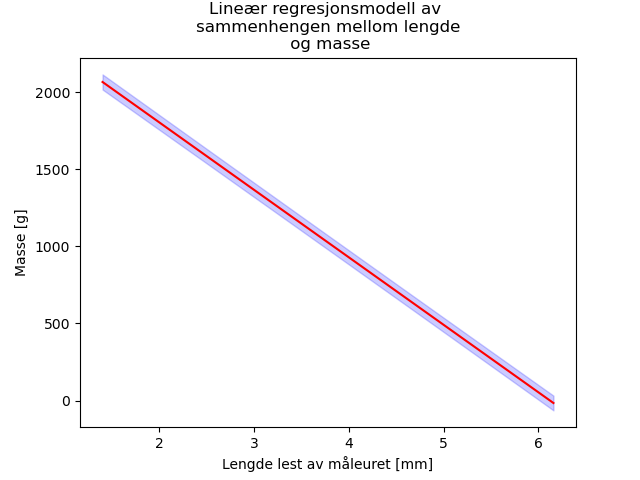
\includegraphics[scale=0.7]{Figurer/Lab_2_regresjon_prediksjon.png}
\end{center}

Programmet ga oss også usikkerhetene for store og små masser:
\begin{center}
\begin{tabular}{  | c | c |}
    \hline
    $u_{\text{små}}$ & 95.8\\
    \hline
    $u_{\text{store}}$ & 98.4\\
    \hline
\end{tabular}
\captionof{table}{Usikkerhetene for små og store masser (i gram)}
\end{center}

Vi kan da altså ikke måle masser under 95.8 gram.

Programmet ga oss også det dynamiske området, som var 1.34.

\subsubsection*{Forsøk e}

Mål for pendelens periodetider ligger vedlagt som vedlegg \ref{Perioder.txt}. Vårt mål av aluminumsloddet ble 2145g. Programmet lagt ved som \ref{Perioder.py} estimerte snittet av disse periodene, samt standardavviket. Programmet ga oss også standardfeil for disse målingene.

\begin{center}
\begin{tabular}{  | c | c |}
    \hline
    $\overline{t}$ & 0.406\\
    \hline
    $s_t$ & 0.0230\\
    \hline
    $SEM(t)$ & 0.00488\\
    \hline
\end{tabular}
\captionof{table}{Snitt, standardavvik, og standardfeil for pendelens periodetider (i sekunder).}
\end{center}

Så snur vi på formel \ref{periodformula} for å estimere k, ved hjelp av snitt-tiden og massen vi målte fra aluminiumsloddet. Dette gir oss:

\begin{align*}
    k &= \frac{4m\pi^2}{\overline{t}^2}\\
      &= \frac{4\cdot 2.145 \cdot \pi^2}{0.406^2} \; \text{kg/$s^2$}\\
      &= 513 \; \text{kg/$s^2$}
\end{align*}

Ved hjelp av formel \ref{gu} (og formel \ref{periodformula}) kan vi finne et uttrykk for usikkerheten i massen:

\begin{align*}
    u_m &= \frac{\overline{t}\cdot k \cdot SEM(t)}{2\cdot\pi^2}\\
    &= \frac{0.406 \cdot 513 \cdot 0.00488}{2\cdot \pi^2}\\
    &= 0.0515 \; \text{kg}\\
    &= 51.5 \; \text{g}
\end{align*}

Mål for periodetidene med $u_m, 2u_m$ og $3u_m$ tilsatt ligger også i vedlegg \ref{Perioder.txt}.
Disse periodetidene, plottet sammen med de originale periodetidene, ser slik ut:

\begin{center}

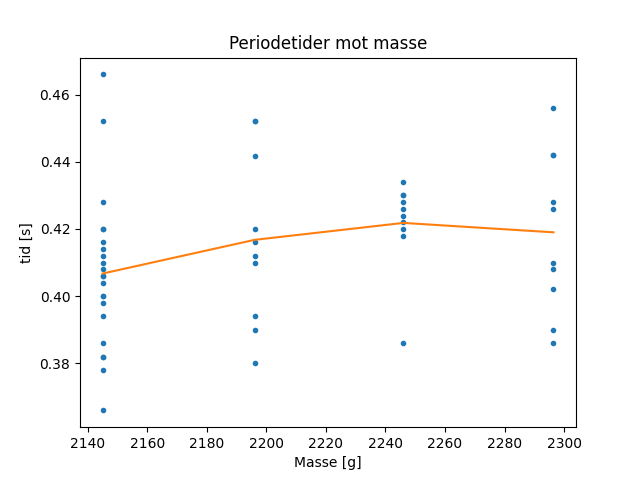
\includegraphics[scale = 0.45]{Figurer/Lab_2_Masse_Mot_Periode.png}
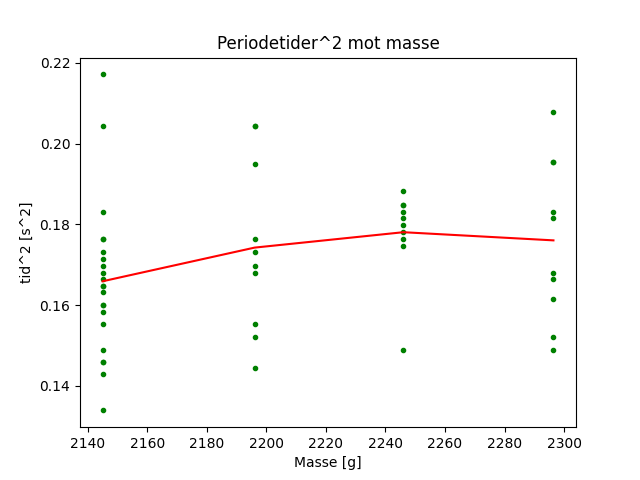
\includegraphics[scale = 0.45]{Figurer/Lab_2_Masse_Mot_Periode2.png}

\captionof{figure}{Plott av periodetid mot masse, sammen med snittet for hver masse. Her plottet med tid (venstre) og $\text{tid}^2$ (høyre).}
\label{MassePeriode}
    
\end{center}

\subsection{Diskusjon}

\subsubsection*{Forsøk d}

Vi så allerede ved andre mål at vekten ikke kunne måle masseforskjeller under 1g, og valgte dermed ikke å måle så små masseforskjeller. Vi valgte også ikke å måle høyere masser enn 2100, og når vi så brukte regresjonsmodellen vår til å finne massen til aluminiumsloddet, fant vi ut at aluminiumsloddet hadde høyere masse enn det vi målte med kalibreringsloddene. Vi har altså at aluminumsloddets masse er utenfor området vi har modellert, og vi kan dermed ikke være veldig sikre på tallet. \smallskip

Selv om vi ikke kan være veldig sikre på tallet, målte vi vekten til aluminiumsloddet for forsøk e, og vet dermed at vår estimerte masse er ganske nærme.\smallskip

Vi valgte å plotte masse mot lengde, som ga oss en omvendt proporsjonalitet mellom dem, men det hadde vært mer hensiktsmessig å ha differansen mellom lengden lest av måleuret uten masse og lengden lest av måleuret med masse på x-aksen. Denne differansen ville gått opp med massen, og vi hadde dermed fått en direkte proporsjonalitet i stedet. Dersom vi skulle gjennomført forsøket igjen, ville vi sannsynligvis gjort dette.\smallskip

Fra residualplottet kunne vi se et systematisk avvik, både mot midten av grafen og i endene. Dette kan selvsagt bety at vi kalibrerte feil, men mer sannsynlig er det noe feil i antakelsen vår om at massen og lengden er proporsjonale. \smallskip

Prediksjonsintervallet ga oss usikkerhetene i små og store masser, og disse usikkerhetene er relativt store. For små masser har vi også målt forskjeller på under 95.8g, som betyr at disse usikkerhetene ikke er helt riktige. Hadde vi hatt tid, hadde vi sjekket dette for store masser også. Feilen i usikkerhetene kan komme fra [HVA DA???] \smallskip

Til slutt i eksperimentet skulle vi måle aluminiumsloddet igjen sammen med en liten masse lik usikkerheten. På grunn av dårlig tid fikk vi ikke gjort dette.

\subsubsection*{Forsøk e}

Vi hadde ikke mulighet til å måle en og en periodetid, pendelen svingte fortere enn vi klarte å reagere. Dette er grunnen til at vi valgte å måle fem og fem svingninger, og så dele på fem etterpå. 
Aluminiumsloddet vi brukte til å anslå pendelens masse, var ikke det samme som loddet festet til pendelen. Dette introduserer selvsagt en usikkerhet, men vi valgte å neglisjere denne. \smallskip

Når vi fant konstanten $k$, antok vi at denne konstanten var idealistisk, altså at den riktig, og ikke endrer seg. Dette er den eneste måten vi kan bruke den samme formelen for å finne usikkerheten i massen. \smallskip

På plottet av periodetid mot masse, kan vi se at snittet av tidene vokser når massen vokser, i hvert fall for de to første masseøkningene. Dette tyder mot at vi kan bruke en pendel til å måle endringer i masse, men også kanskje at våre mål er for unøyaktige til å gjøre dette ordentlig. Vi begynte å få dårlig tid mot slutten av dette eksperimentet, som kan forklare dette.

\newpage

\section{Ioniserende stråling}

\subsection{Innledning}

Det tredje eksperimentet handlet om ioniserende stråling og radioaktivitet. Hensikten med eksperimentet var å lære om hvordan observert strålingsmengde innen ett tidsintervall er påvirket av statistisk spredning, hvordan stråling blir absorbert, og bruk av Geiger-M$\ddot{\text{u}}$ller-teller. \medskip

Eksperimentet bygger på teori rundt stråling og radioaktivitet. I eksperimentet bruker vi $\gamma$-stråling med høy energi, en form for ioniserende elektromagnetisk stråling. Denne strålingen oppstår som et produkt av noen typer radioaktiv henfall, som er slik vi vil danne denne strålingen.

For en radioaktiv kjerne, vil det være en konstant sannsynlighet for desintegrasjon. En kjerne er enten desintegrert, eller ikke, som betyr at desintegrasjonen følger en Bernoulli-prosess, og fordi sannsynligheten for at kjernen desintegrerer er liten (for mange isotoper) kan vi finne sannsynligheten for et X antall desintegrasjoner over tiden $\Delta$t ved hjelp av en Poissonfordeling.

For dette eksperimentet vil vi bruke en Geiger-M$\ddot{\text{u}}$ller-teller, et instrument som måler antall ioniserte partikler. GM-telleren har et GM-rør, som plukker opp den ioniserende strålingen. 
Noe av denne strålingen (ca 1\%) vil treffe veggen på innsiden av røret og slå løs elektroner via fotoelektrisk effekt. Disse elektronene ioniserer gass-molekylene som befinner seg innad i GM-telleren, og GM-telleren kan måle dette. På denne måten kan vi få et mål på hvor intens en stråling er.\medskip

Formålet med eksperimentet var å måle og analysere dempning av ioniserende stråling gjennom en
absorbator med varierende tykkelse. Vi brukte bly som absorbator, og GM-telleren til å måle dempningen.

\subsection{Material og Metoder}

Til eksperimentet trengte vi Geiger-M$\ddot{\text{u}}$ller-teller (se fig \ref{GM}), radioaktiv kilde , en stoppeklokke (vi brukte mobiltelefon), en mobiltelefon som kan ta opp slow-motion video, skyvelære, og 6 blyplater.\medskip

\bigskip \hfil
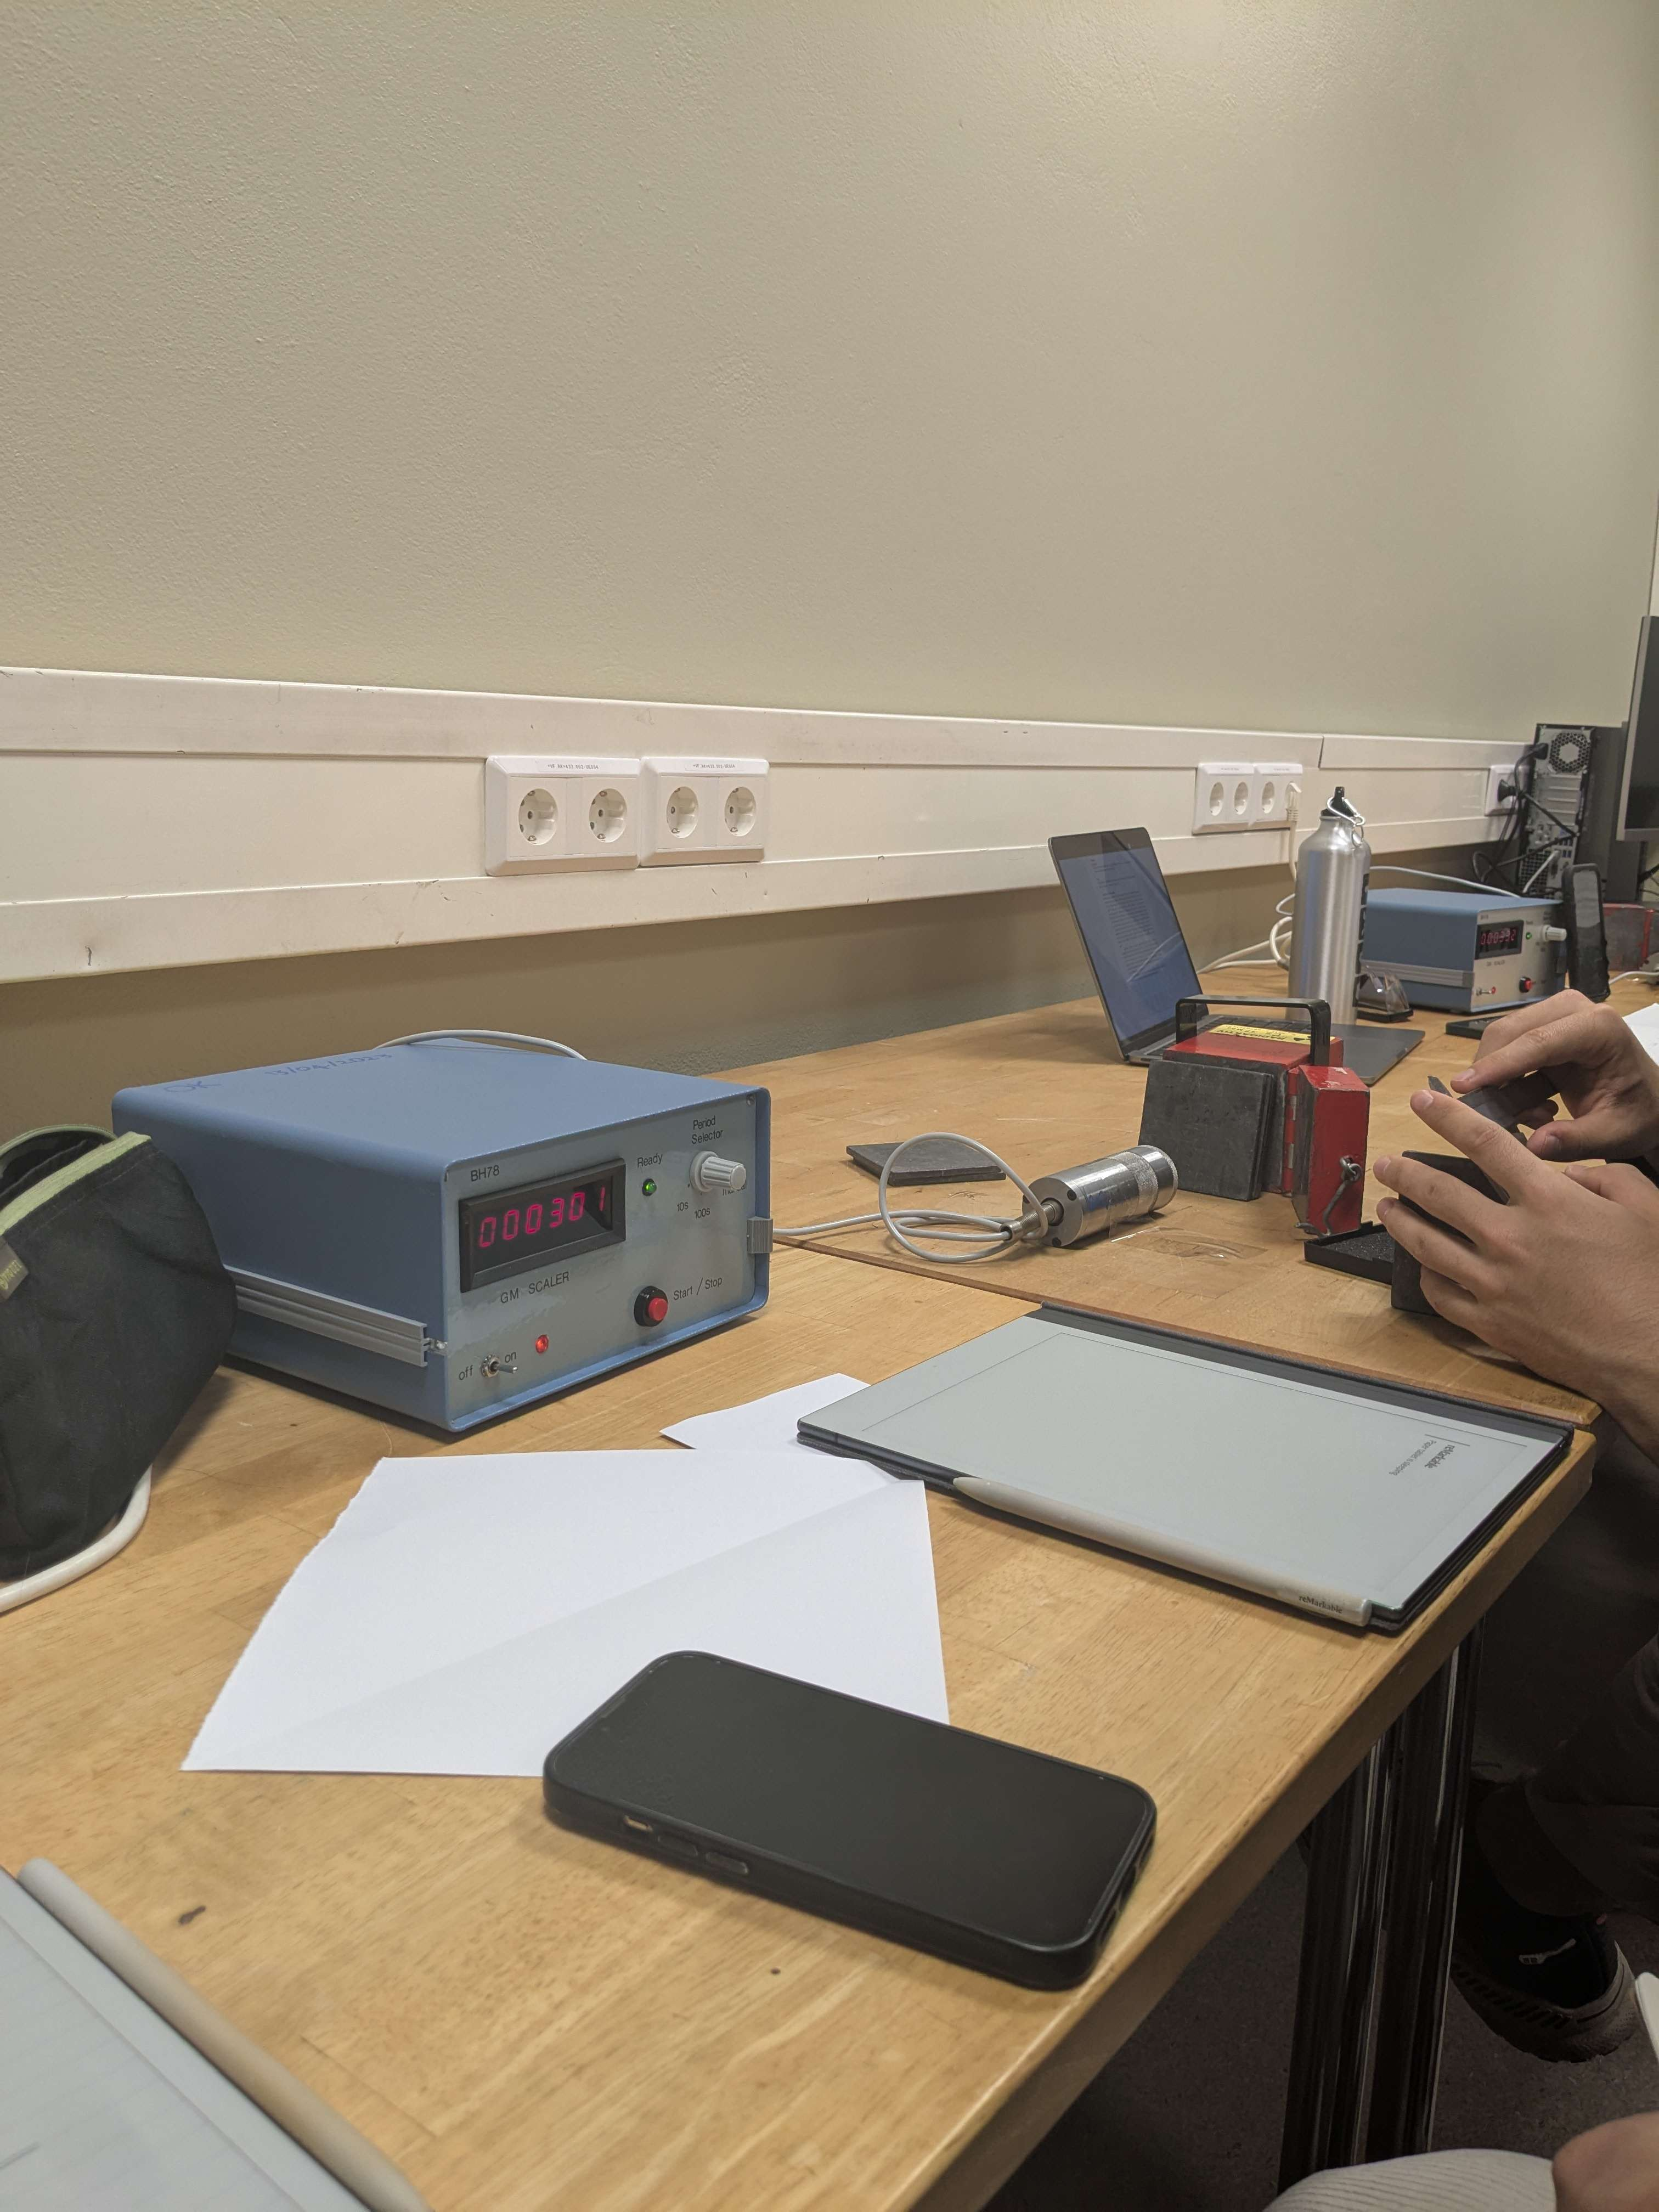
\includegraphics[scale = 0.05]{Figurer/GM-Counter.jpg} 
\captionof{figure}{Geiger-M$\ddot{\text{u}}$ller-telleren (blå), sammen med radioaktiv kilde (rødt), pekende mot GM-rør.}\label{GM}
\par \bigskip

Vi begynte med å måle bakgrunnstrålingen $I_b$. Vi plasserte alle 6 blyplatene foran GM-røret, skrudde på telleren uten noen radioaktiv kilde, og lot den stå på i 10 minutter. Så estimerte vi usikkerheten til $I_b$ ved å bruke at strålingen er Poisson-fordelt. Dette gir oss

\begin{align}
    u_{I_b} = \sqrt{I_b}  \label{u_b}
\end{align}

Vi brukte dette som bakgrunnsstrålingen fremover. \medskip

Så plasserte vi den radioaktive kilden vår foran GM-røret, og sørget for at det ikke bevegde seg under eksperimentet. Vi tok så 5 mål av hvor lang tid det tok for GM-telleren å samle 1000 tellinger, og fant snittet av disse målene. Etter dette, målte vi antall tellinger over snittiden for 1 - 6 blyplater. Før vi målte antall tellinger, målte vi tykkelsen på blyplaten vi la til. Siden tiden $\overline{t}$ var kort, plasserte vi stoppeklokken vår (mobiltelefon) ved siden av GM-telleren, og filmet telleren og klokken i slow-motion, slik at vi kunne plukke ut tiden mer nøyaktig.\medskip

For å finne usikkerheten i en sum av andre usikre variabler, brukte vi følgende formel
\begin{align}
    u_f = \sqrt{u_x^2 +u_y^2}\label{au2}
\end{align}

Mer generelt anvendte vi 

\begin{align}
    u_f^2 = \left(\frac{\delta f}{\delta x} u_x\right)^2 + \left(\frac{\delta f}{\delta y} u_y\right)^2\label{gu3}
\end{align}

Vi fant også relative usikkerheter ved følgende formel:
\begin{align}
    r_x = \frac{u_x}{\sqrt{x}}
\end{align}


Til slutt, plottet vi Strålingen mot blytykkelsen i python. Vi plottet også Strålingen log-transformert, slik at den ble lineær med blytykkelsen. For å gjøre dette, brukte vi følgende sammenheng:

\begin{align}
    I = I_0e^{-\mu_\gamma x} \implies \ln{I} = -\mu_\gamma x + \ln{I_0}\label{stbt}
\end{align}

Der $I_0$ er strålingen uten noen blyplater, og $\mu_\gamma$ er dempningskoeffisienten. 

\subsection{Resultater}

Bakgrunnstrålingen $I_b$ i løpet av 10 minutter ble målt til 266. Formel \ref{ub} gir oss da $u_{I_b} = \sqrt{266} = 16,31$. Dette bruker vi som bakgrunnsstrålingen fremover. \medskip

Våre fem mål for tiden GM-telleren brukte på å samle 1000-tellinger uten noen blyplater, samt snittet av disse, ble som følger:

\begin{center}
\begin{tabular}{ | c | }
    \hline
    t\\ 
    \hline
    14.05\\ 
    \hline
    14.28\\ 
    \hline
    14.76\\ 
    \hline
    14.56\\ 
    \hline
    15.46\\ 
    \hline
\end{tabular}\;\;\;
\begin{tabular}{ | c | }
    \hline
    $\overline{t}$\\ 
    \hline
    14.622\\ 
    \hline
\end{tabular}
\captionof{table}{Målte tider for 1000 tellinger uten blyplater, sammen med snittet av disse tidene (i sekunder).}
\end{center}

Tykkelsen på de 6 blyplatene:

\begin{center}
\begin{tabular}{ | c | c | }
    \hline
    & dx\\ 
    \hline
    1 & 0.53\\ 
    \hline
    2 & 0.32\\ 
    \hline
    3 & 0.525\\ 
    \hline
    4 & 0.52\\ 
    \hline
    5 & 0.51\\ 
    \hline
    6 & 0.511\\ 
    \hline
\end{tabular}
\captionof{table}{Tykkelsen på de 6 blyplatene (i cm)}
\end{center}

Den samlede tabellen med alle mål tatt av GM-telleren:

\begin{center}
\begin{tabular}{ | c | c | c | c | c | }
    \hline
    Antall blyplater & Total Blytykkelse dx (cm) & $u_{dx}$ (cm) & Antall Målinger & standardavvik\\ 
    \hline
    1 & 0.53 & 0.0071 & 604 & 24.58\\ 
    \hline
    2 & 0.83 & 0.01 &381 & 19.52\\ 
    \hline
    3 & 1.38 & 0.012 &269 & 16.40\\ 
    \hline
    4 & 1.90 & 0.014 &130 & 11.40\\ 
    \hline
    5 & 2.40 & 0.016 &86 & 9.27\\ 
    \hline
    6 & 2.92 & 0.017 &42 & 6.48\\ 
    \hline
\end{tabular}
\captionof{table}{Antall blyplater, Totale blytykkelser, usikkerhet i disse blytykkelsene, antall målinger fra GM-telleren, og standardavvikene for disse målene.} \label{bigtable}
\end{center}

standardavvikene her er funnet fra formel \ref{u_b}, og usikkerhetene er funnet fra skyvelærens skalausikkerhet $u_{skala} = 0.05$ mm, skyvelærens avlesningsusikkerhet $u_{avles} = 0.05$ mm, og formel \ref{au2}.

Relative Usikkerheter for Blytykkelse og Antall målinger:

\begin{center}
\begin{tabular}{ | c | c | c |}
    \hline
    N plater & $r_x$ &  $r_n$\\ 
    \hline
    1 & 0.009753 & 1.0001\\ 
    \hline
    2 & 0.01097 & 1.0000\\ 
    \hline
    3 & 0.01021 & 0.9999\\ 
    \hline
    4 & 0.01015 & 0.9998\\ 
    \hline
    5 & 0.01032 & 0.9996\\ 
    \hline
    6 & 0.009948 & 0.9998\\  
    \hline
\end{tabular}
\captionof{table}{Relative usikkerheter for blytykkelse og antall målinger} 
\end{center}

Vi fikk følgende plott for Stråling mot blytykkelse:

\begin{center}
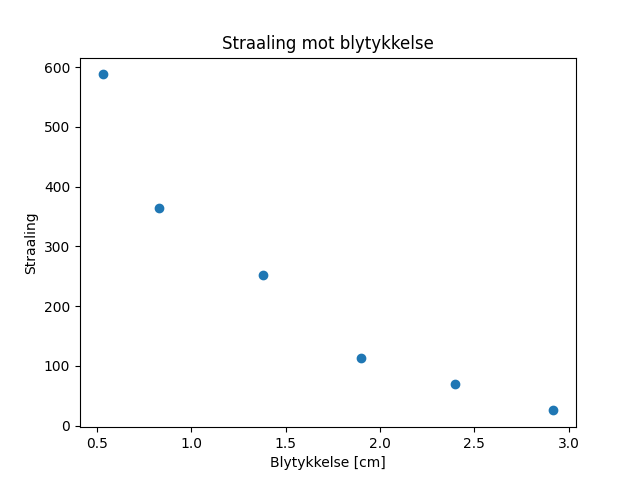
\includegraphics[scale=0.7]{Figurer/Straaling_Bly.png}
\end{center}

Så for log-transformerte data (ved bruk av formel \ref{stbt}):

\begin{center}
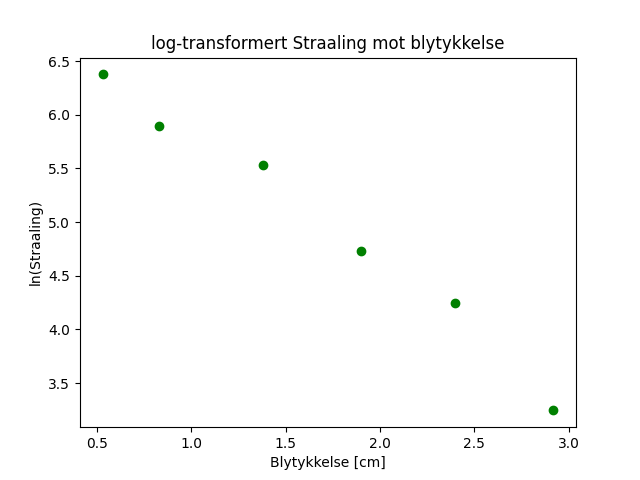
\includegraphics[scale=0.7]{Figurer/LogStraaling_Bly.png}
\end{center}

Vi tilpasset en lineær regresjonsmodell til dette plottet:

\begin{center}
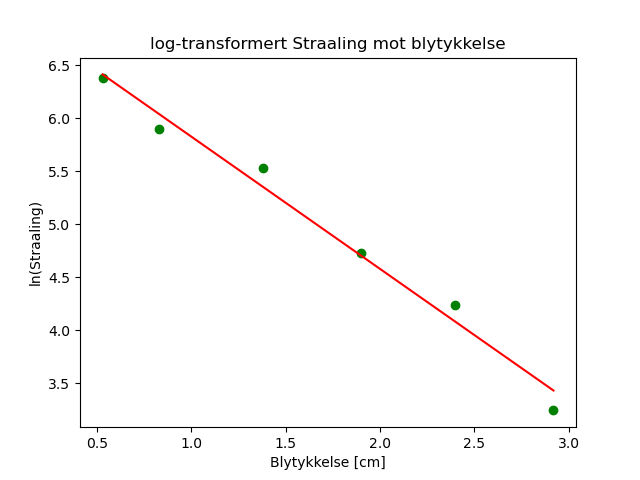
\includegraphics[scale=0.7]{Figurer/LogStraaling_Regresjon.png}
\end{center}

Denne regresjonsmodellen ga oss et uttrykk for  $\ln{I}$, og usikkerhetene i $\beta_0$ og $\beta_1$. Sammen med formelog $u_{\n{I}}$:

\begin{align*}
    (\ln{(I)})(x) &= -1.247014\cdot x + 7.075217\\
    u_{\n{I}} &= \sqrt{(x\cdot 0.082)^2 + 0.153^2}
\end{align*}

Programmet ga oss også et estimat for blytykkelsen nødvendig for at 90\% og 99\% av strålingen skal absorberes:

\begin{center}
\begin{tabular}{ | c | c | c | }
    \hline
    Prosentandel & 90\% & 99\%\\ 
    \hline
    Blytykkelse & 5.107 & 5.617\\ 
    \hline
    Usikkerhet & 0.4458 & 0.48534\\ 
    \hline
\end{tabular}
\captionof{table}{Nødvendig blytykkelse (i cm) for å absorbere 90\% og 99\% av strålingen.}
\end{center}

[Usikkerhet for dette!!!]

\subsection{Diskusjon}

Selv om det ikke ble spesifisert i oppgaven, valgte vi å ta flere mål av tiden GM-telleren brukte på å samle 1000 tellinger, og når vi da bruker snitt-tiden, får vi et noe mer nøyaktig mål (ideelt sett skulle vi hatt flere målinger av t).\medskip

Målene våre for blyplatenes tykkelser er ganske nøyaktige, grunnet skyvælærens lave usikkerheter. Når vi ser på en sammenheng som dette, der både tykkelsene og tellingene er usikre, kan vi se i tabell \ref{bigtable} at dersom vi bruker tellingenes standardavvik som usikkerheter, at disse er mye større enn usikkerhetene for for tykkelsen i platene. Samtidig øker usikkerheten i tykkelsene med antall plater, mens usikkerheten i tellingene minker, så om den totale blytykkelsen blir stor, kan dette forholdet endres.\medskip

[Noe om relativ usikkerhet???]\medskip

I det første plottet, der stråling plottes direkte mot blytykkelse, ser vi punkter som danner en kurve som blir mindre bratt når blytykkelsen øker. Dette samsvarer med formel \ref{stbt}, hvor vi kan se at I er omvendt proporsjonal med $e^x$, som danner en graf som ser slik ut.

I det andre plottet, der $\ln{I}$ plottes mot blytykkelsen, får vi punkter som danner en rett linje. Dette samsvarer igjen med formel \ref{stbt}, der vi kan se at $\ln{I}$ er lineær med x. Sammen med utrykket vi fikk fra regresjonen, kan vi også da finne at $\mu_\gamma$ er stigningen i dette utrykket, 1.247014. Samtidig er ikke denne modellen helt perfekt. Det lineære utrykket gir oss at $\ln{I_0} = 7.075217$, som gir oss $I_0 = e^{7.075217} = 1096.6$, som ikke er helt nøyaktig. Dette kunne bli løst med flere blyplater, som kunne gitt oss en bedre modell. Vi kunne også fått en bedre modell ved å måle tellinger for flere kombinasjoner av platene, i stedet for å kun måle i rekkefølge.\medskip

[Noe om å lære å bruke GM-teller??]


\newpage

\section{Prosjektil}

\subsection{Innledning}

Det fjerde og siste eksperimentet handlet om en prosjektilbevegelse. Dette er en bevegelse der et objekt skytes ut i luften, og kun påvirkes av akselerasjon gjennom tyngdekraften. Vi ser dermed bort fra luftmotstand i dette eksperimentet.

I en slik situasjon er bevegelsene på x- og y-aksen uavhengige, og vi kan regne med dem hver for seg. Det er dermed ingen akselerasjon i bevegelsen på x-aksen, mens y-aksen kun påvirkes av gravitasjonsakselerasjonen. Ved å vite dette kan vi ved hjelp av noen målinger finne ut mye om bevegelsen. Sentralt ligger bevaring av energi og de enkleste bevegelseslikningene.

Bevegelser som dette dukker opp ofte i fysikken. Vi vil ta for oss en prosjektilbevegelse i to dimensjoner, men en slik bevegelse kan beskrives i flere dimensjoner også

\subsection{Material og Metoder}

For eksperimentet trengte vi en prosjektilskyter (se fig \ref{projectile}), en prosjektil å skyte, en målestokk, 2 vanlige ark, et ark karbonpapir, og en mobiltelefon.

\bigskip \hfil
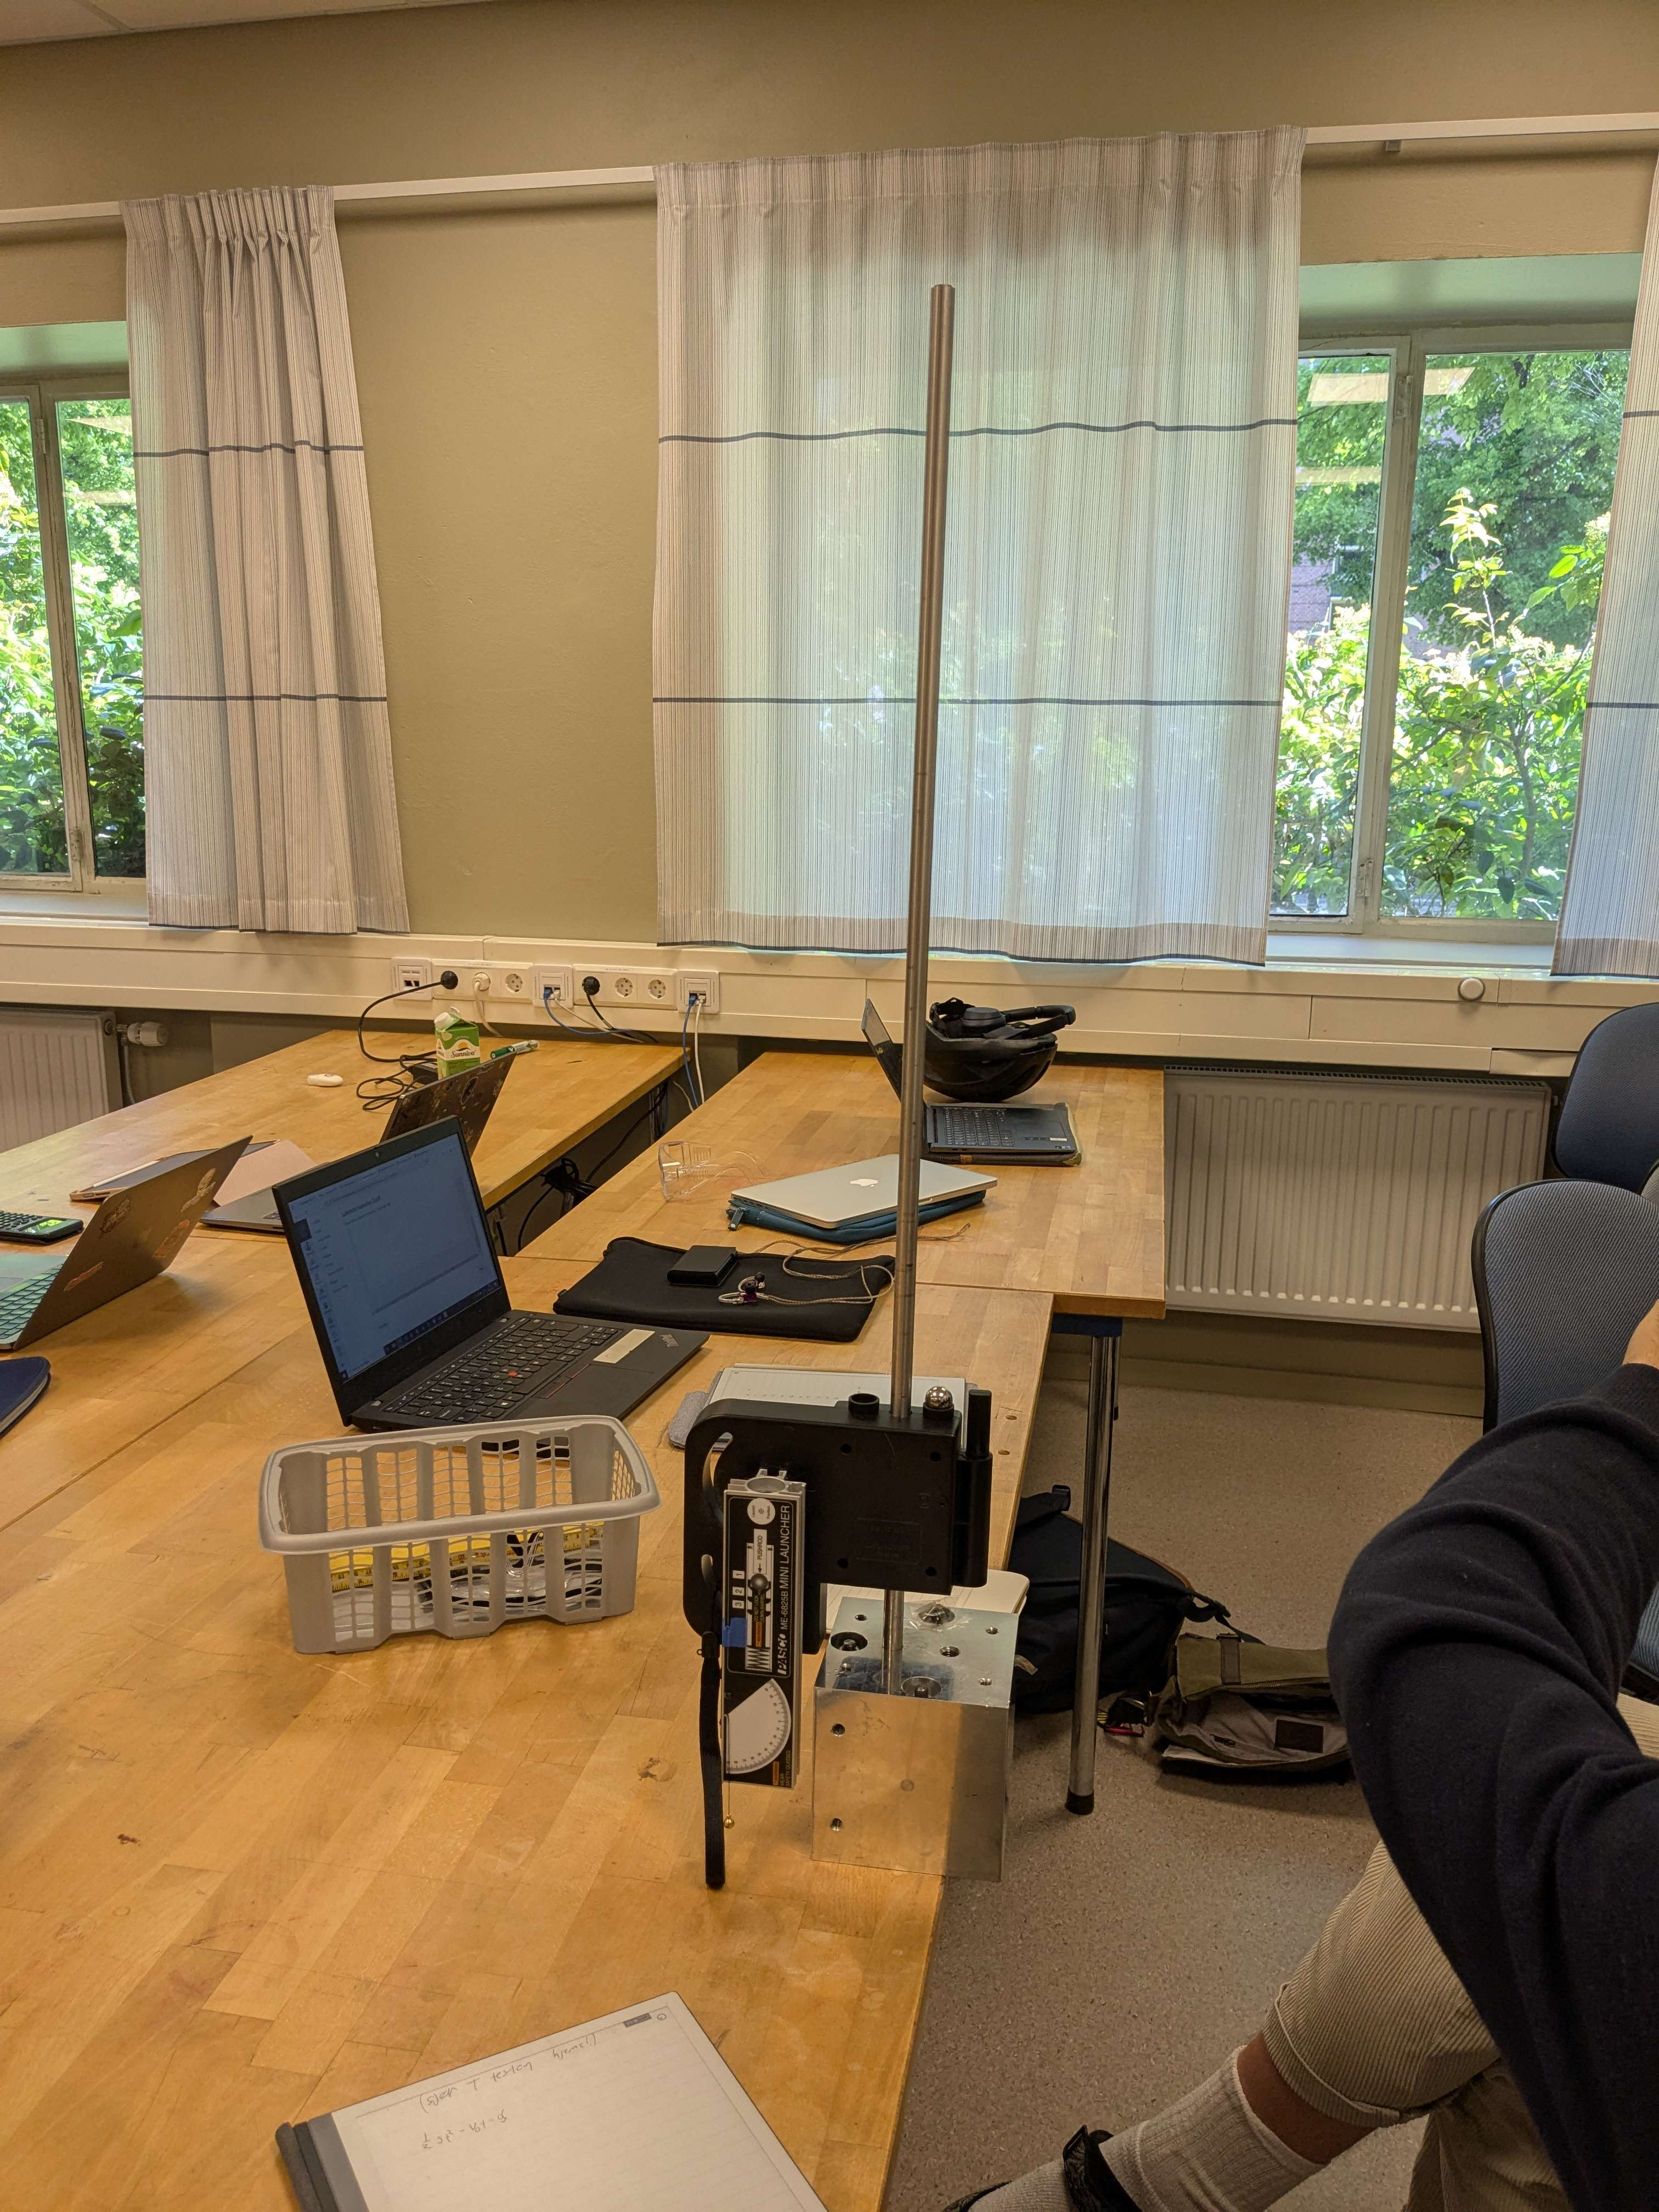
\includegraphics[scale = 0.05]{Figurer/Projectile.jpg} 
\captionof{figure}{Prosjektilskyteren}\label{projectile}
\par \bigskip

Først orienterte vi skyteren slik at prosjektilbevegelsen skulle bli et horisontalt kast, og så målte vi høyden fra bordet til prosjektilskyteren. Vi estimerte tiden dette kastet ville ta med følgende formel:

\begin{align}
    \hat{t} = \sqrt{\frac{2h_0}{g}}\label{that}
\end{align}

Så utførte vi en t-test for å sjekke om vi kunne måle tiden i et slikt kast. Vi brukte følgende formel for t-testen:

\begin{align}
    T = \left|\frac{t_{reaksjon} - \hat{t}}{u_{t_{reaksjon}}}\right|\label{ttest}
\end{align}

\medskip

Så orienterte vi skyteren slik at kastet ville bli kun vertikalt. Ved å måle det høyeste punktet prosjektilen når, kan vi bruke bevaring av energi

\begin{align}
    v_0 = \sqrt{2gh}\label{energy}
\end{align}

til å finne startfarten. Vi tok 20 mål av prosjektilens maksimale høyde. Vi gjorde dette ved å stille opp målestokken langs med prosjektilskyteren, skyte prosjektilen fra første hakk i skyteren, og filme området der prosjektilen var på sitt høyeste i slow-motion video, med mobiltelefonen. Slik kunne vi ganske nøyaktig plukke ut høyden. \medskip

Når vi hadde 20 mål for høyden, fant vi snittet av disse, og brukte det til å estimere starthastigheten. Vi brukte python for å gjøre dette. Programmet ga oss også et estimat for rekkevidden til et kast ved $\theta = 30^\circ$. Vi gjorde dette ved å først finne tiden (se formel \ref{timeformula}), og så hvor langt prosjektilen vil bevege seg på x-aksen (se formel \ref{xformula}):

\begin{align}
    t &= \frac{\sin{\theta}\cdot v_0 + \sqrt{(\sin{\theta})^2\cdot v_0^2 + 2gh_0}}{g} \label{timeformula}\\
\end{align}
\begin{align}
    x &= \cos{\theta}\cdot v_0 \cdot t \label{xformula}
\end{align}

Når vi hadde dette estimatet, orienterte vi skyteren slik at vi ville få et kast med $\theta = 30^\circ$. Så målte vi strektning lik rekkevidden vi hadde estimert, teipet vi et hvitt ark på bordet, og markerte estimatet vårt for rekkevidde på arket. Så plasserte vi karbonpapiret på toppen av det hvite arket, og så enda et hvitt ark på toppen av dette. Vi teipet så alle arkene ned til bordet. Så gjennomførte vi kastet med $\theta = 30^\circ$ 19 ganger, slik at prosjektilen landet på papirene. Når vi så tok av de to øverste arkene, hadde karbonpapiret markert hvor prosjektilen landet, slik at vi kunne måle hvor langt de hadde beveget seg.\medskip

Når vi målte strektningen for å plassere papiret, målte vi fra siden av skyteren, og ikke fra utskytningspunktet. Vi måtte dermed korrigere for det (se fig \ref{ProjDiagram})

\bigskip \hfil
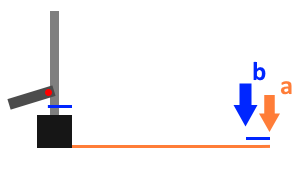
\includegraphics[scale = 0.5]{Figurer/ProsjektilDiagram.png} 
\captionof{figure}{a er strektningen vi målte til, som er litt for lang. b er den ordentlige strektningen fra utskytningspunktet, estimert i programmet.}\label{ProjDiagram}
\par \bigskip

Til slutt fant vi snittet av alle rekkeviddene vi målte, utførte en t-test for å sjekke om estimatet vårt var riktig, og plottet dataen. Formelen vi brukte for denne t-testen var:

\begin{align}
    T = \left|\frac{\overline{x} - \hat{x}}{SEM(x)}\right|\label{ttest2}
\end{align}

For å finne usikkerheten i en sum av andre usikre variabler, brukte vi følgende formel
\begin{align}
    u_f = \sqrt{u_x^2 +u_y^2}\label{au3}
\end{align}

Mer generelt anvendte vi 

\begin{align}
    u_f^2 = \left(\frac{\delta f}{\delta x} u_x\right)^2 + \left(\frac{\delta f}{\delta y} u_y\right)^2\label{gu2}
\end{align}

\subsection{Resultater}

Måle vårt for høyden på skyteren ble som følger:

\begin{center}
\begin{tabular}{ | c | c | }
    \hline
    $h_0$ & $u_{h_0}$ \\ 
    \hline
    21.4 & 0.0866\\ 
    \hline
\end{tabular}
\captionof{table}{Mål på utskytningspunktets høyde (i cm). Usikkerheten er funnet fra målestokkens skala- og ledd-usikkerhet, og en avlesningsusikkerhet. Alle disse var på 0.05cm, og $u_{h_0}$ ble funnet fra formel \ref{au3}}
\end{center}

Fra formel \ref{that} fikk vi $\hat{t} = 2.09$ s.  t-testen gir oss da $T = 8.2$, der grensen er $6.314$ for $T_{95}$ \medskip

Vi fikk 20 målinger for prosjektilens høyde i det vertikale kastet. Disse ligger i vedlegg \ref{Heights.txt}.

Programmet (vedlegg \ref{Get_h_line.py}) ga oss følgende estimater:

\begin{center}
\begin{tabular}{ | c | c | c | c | }
    \hline
    $\overline{h}$ (cm) & $v_0$ (m/s) & $\hat{t}$ (s) &  $\hat{x}$ (cm) \\ 
    \hline
    60.25 & 3.44 & 0.45 & 133 \\      
    \hline
\end{tabular}
\captionof{table}{Estimater fra programmet. Fra venstre til høyre: Snitthøyden i det vertikale kastet, startfarten estimert fra snitthøyden, den estimerte tiden i kastet med $\theta = 30^\circ$, og estimert distanse langs x-aksen i dette kastet.}
\end{center}

Mål på rekkeviddene i bevegelsen med $\theta = 30^\circ$ ligger vedlagt som vedlegg \ref{Lengths.txt}. Merk at avstandene er fra vårt estimat for rekkevidden, og ikke fra utskytningspunktet. Programmet lagt ved som vedlegg \ref{WorkWithLengths.py} ga oss følgende snittrekkevidde og usikkerhet:

\begin{center}
\begin{tabular}{ | c | c |  }
    \hline
    $\overline{x}$ & $SEM(x)$\\ 
    \hline
    $135.44$ & 0.093\\     
    \hline
\end{tabular}
\captionof{table}{Snittrekkevidde og usikkerhet i kast med $\theta = 30^\circ$, i cm.}
\end{center}

t-testen ga oss da T = 26.25, der grensen er 6.314 for $T_{95}$. \medskip

Programmet lagt ved som vedlegg \ref{WorkWithLengths.py} plottet også lengdene sammen med estimert rekkevidde:

\bigskip \hfil
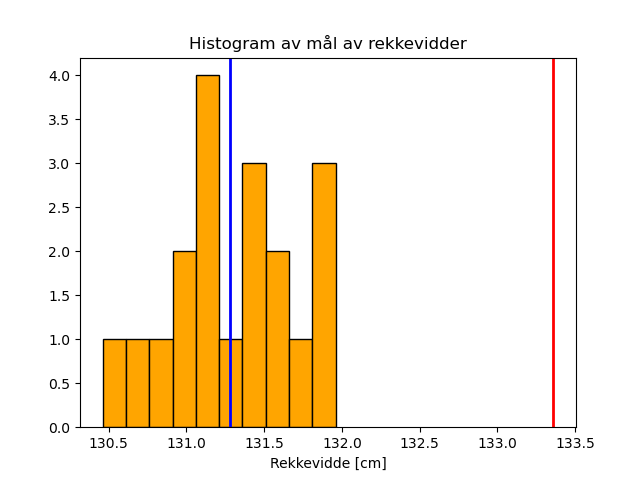
\includegraphics[scale = 0.75]{Figurer/HistRekkevidde.png} 
\captionof{figure}{Histogram av målte rekkevidder, sammen med estimert rekkevidde (rød) og snittrekkevidde (blå)}\label{RekkeviddeDiagram}
\par \bigskip


\subsection{Diskusjon}

Til og med før vi gjennomførte t-testen skjønte vi at vi ikke kunne måle tiden i det horisontale kastet, siden vi ikke ville reager i tide. t-testen bekreftet dette. Derfra valgte vi et vertikalt kast, slik at vi ikke må tenke på vinkler. 

Akkurat som i eksperiment 3 brukte vi slow-motion video til å finne høyden i det vertikale kastet. Dette kommer med begrensningen at mobiltelefonen har en grense på hvor mange bilder den kan ta i sekundet, men er fortsatt en mer nøyaktig måte å måle på enn øyemål.\medskip

For de målte rekkeviddene, kan vi se på histogrammet at estimatet er lenger vekk fra utskytningspunktet enn målene. Dette skyldes en systematisk feil sikkert :)

Noe om systematiske feil???

\newpage

\section{Konklusjon}

Fikse REF!!!

Referer til oppgavebeskrivelsene

\newpage

\section{Referanser}

\newpage

\section{Vedlegg} \label{Vedlegg}

Svingetid.txt
\label{Svingetid.txt}

Svingehistogram.py \label{Svingehistogram.py}

SEM.py \label{SEM.py}

Kalibreringskurve.py \label{Kalibreringskurve.py}

Perioder.txt
\label{Perioder.txt}

Perioder.py
\label{Perioder.py}

IntensityPlot.py
\label{IntensityPlot.py}

TrueIntensity.txt
\label{TrueIntensity.txt}

Get\_h\_line.py
\label{Get_h_line.py}

Heights.txt
\label{Heights.txt}

Lengths.txt
\label{Lengths.txt}

WorkWithLengths.py
\label{WorkWithLengths.py}

\end{document}
